\documentclass[12pt]{article}
\usepackage{amsfonts}
\usepackage{amsmath}
\usepackage{algorithm2e}
\usepackage{graphicx}
\usepackage{boxedminipage}
\usepackage{fancybox}
\usepackage{eucal}
\usepackage{theorem}
\usepackage{natbib}



\setlength{\textheight}{1.01\textheight}
\newtheorem{thm}{Theorem}[section]
\theoremstyle{plain}
\newtheorem{definition}[thm]{Definition}
\newtheorem{lem}[thm]{Lemma}
\newtheorem{pro}[thm]{Proposition}
\newtheorem{cor}[thm]{Corollary}

\def\Zp{{\mathbf{Z}^+}}
\def\Zk{{\mathbf{Z}_{\kappa}}}
%\def\tk{{T^{(\kappa)}}}

\setlength{\parskip}{6pt}
\begin{document}

\title{Baysian-Glasso model for stock return series analysis}

\author{Jian wang  and Jinfeng Zhang}
\date{\today}

\maketitle

\begin{abstract}
Structure learning process always stands an important problem in the Bayesian network research area.In this paper, we applied the Grphic Lasso(Glasso) model into the Bayesian network structure learning area. Most Bayesian network structure learning algorithms,such as hill climbing algorithm, started from a random graph and adjusted the direction of edges to obtain the optimal graphic structure. We tried to use the result of the GLasso model as the start graphic and learnt the optimal structure based on this initial network. The program language that we used for this research was R and the two major packages in our research were "Bnlearn" and "Huge". Besides, we also applied this Bayesian-Glasso model into stock return series analysis and compared the BIC score for different models. We found that in the stock return study area, the performance is better for the Bayesian-Glasso model than the bayesian network model itself. To our knowledge, it is the first time to apply the Glasso model into the Bayesian network structure learning area.

\end{abstract}

\section{Introduction}

The Bayesian network is a probabilistic graphic model that represents a set of random variables and their conditional dependencies via the directed acyclic graph(DAG). Each node in the graph represents a random variable. Each random variable has a set of mutually exclusive and collectively exhaustive possible values. That is, exactly one of the possible values is or will be the actual value, and we are uncertain about which one it is. Bayesian networks are widely used in many areas to create consistent probabilistic representations of uncertain knowledge. For example, in the medicla diagnosis( Spiegelhalter et al., 1989), image recognition (Booker, Hota, 1986), language understanding (Charniak, Goldman, 1989a, 1989b), search algorithms (Hansson, Mayer, 1989). The Bayesian networks provide an elegant mathematical structure for modeling complicated relationships among random variables while keeping a relatively simple visualization of these relationships. There are more literatuer on this topic such as Pearl (1988), Neapolitan (1990, 2003), Oliver \& Smith (1990), Charniak (1991), Jensen (1996, 2001) and  Korb \& Nicholson (2003).\\

There are two main problems in Bayesian network research area. One is the structure learning problem. This problem is trying to find the optimal structure of the network for the random variables that we need to observe. Generally, people used greedy algorithm such as Hill-climbing algorithm to handle this problem. Another important problem is parameter learning. Once the structure of the network has been defined, the next task is to estimate and update the parameters of the global distribution.  Parameter estimation remained problematic in many situations. For example, it is increasingly common to have sample sizes much smaller than the number of variables included in the model. In our paper, we focused on the problem of structure learning for the Bayesian network. Our method was to use the result of the Graphical Lasso model as the initial network and then used the greedy algorithm to learn the structure. \\

The Graphical Lasso was first introduced by Jerome Friedman, Trevor Hastie and Robert Tibshirani(2007), It was introduced by solving the problem of estimating sparse graphs by a lasso penalty applied to the inverse covariance matrix. The most widely used R package for the Glasso problem was called the glasso. In 2012, Tuo zhao and Han Liu describe a new R package named High-dimensional Undirected Graph Estimation(huge) package which provided easy to use functions to estimating the high dimensional undirected graphs from data.  Compared with glasso package, the huge package contains the following features: 1) It was written in C, which was easier to modify. 2) it provided functions for fitting high dimensional semiparametric Gaussian copula models. 3) The package provided both lossless and lossy screening rules to scale up large-scale problems. We used the huge package to build the relationship among the stock returns. Since the Glasso model only gave us the relationship among the random variables, the network was undirected. Hence,we random generated the directions of the existing edges and use this network as initial start for the structure learning process. \\

During the first decade of the 21 century, the economic market shrunk very much. For example the subprime crisis, it resulted in the collapse of many large financial institutions, such as the bankruptcy of the Lehman brothers holding Inc. Hence, it is very important for the investment sectors to build some more efficient and accurate models to manage risk and reduce the future loss to the least level.
Our work is to use bayesian network and Glasso model to find the causal relationship amongs stock return series. The stock data that we used is from the website Yahoo finance. The data from the website yahoo finance contain some variables such as open price, highest price, lowest price,etc. Here we only use the open and close price to calculate the  return series of the daily stock price change.The Glasso model was used to learn the structure of the relationship between the stocks and Bayesian network was used to find the causal network of  the daily stock price. The calculation process is realized by the "Bnlearn" and "Huge" packages of software R.\\

The remaining structure of this paper was as follows: Chapter 2 was the introduction of the Bayesian network and the structure learning algorithm. The basic knowledge of GlASSO model was described in chpter 3. Chapter 4 discussed how we applied the Bayesian network and GLASSO model to analyze the stock return price series. Chapter 5 were some conclusions about our work.


\section{Baeysian network and structure learning process}
Before we introduced the Bayesian network, we first need to know some basic know of graph.\\
A graph $G=(\bf{V},\bf{A})$ consists of a nonempty set $\mathbf{V}$ of $\emph{nodes}$ or $\emph{vertices}$ and a finite (but possibly empty) set $\mathbf{A}$ of pairs of vertices called $\emph{arcs, links, or edges}$.\\
Each arc $\emph{a=(u,v)}$ can be defined either as an ordered or an unordered pair of nodes, which are said to be $\emph{connected}$ by and $\emph{incident}$ on the arc and to be $\emph{adjacent}$ to each other. Since they a re adjacent, $\emph{u}$ and $\emph{v}$ are also said to be $\emph{neighbours}$. If $\emph{(u,v)}$ is an ordered pair,$\emph{u}$ is said to be the $\emph{tail}$ of the arc and $\emph{v}$ is the $\emph{head}$; then the arc is said to be $emph{directed}$ from $\emph{u}$ to $\emph{v}$ and is usually represented with an arrowhead in $\emph{v}(u \rightarrow v)$. It is also said that the arc $\emph{leaves}$ or is $\emph{outgoing}$ for $\emph{u}$ and that it $\emph{enters}$ or is $\emph{incoming}$ for $\emph{v}$. If $\emph{(u,v)}$ is unordered, $\emph{u}$ and $\emph{v}$ are simply said to be incident on the arc without any further distinction. In this case, they are commonly referred to as $\emph{undirected arcs or edges}$, denoted with $\emph{e} \in \mathbf{E}$ and represented with a simple line $\emph(u-v)$.\\
The characterization of arcs as directed or undirected induces an equivalent characterization of the graphs themselves, which are said to be $\emph{directed graphs}$ (denoted with $\emph{G}$=$(\mathbf{V},\mathbf{A})$) if all arcs are directed, $\emph{undirected graphs}$( denoted with $\emph{G}$=$\emph{(V,E)}$ if all arcs are $\emph{undirected}$, and $\emph{partially directed}$ or $\emph{mixed graphs}$ (denoted with $\emph{G}$= $\mathbf{(V,A,E)}$ if they contain both directed and undirected arcs.\\

Figure 1 shows the examples of $\emph{directed, undirected, and mixed partially directed}$ graphs. \\
\begin{figure}[!htb]
\centering
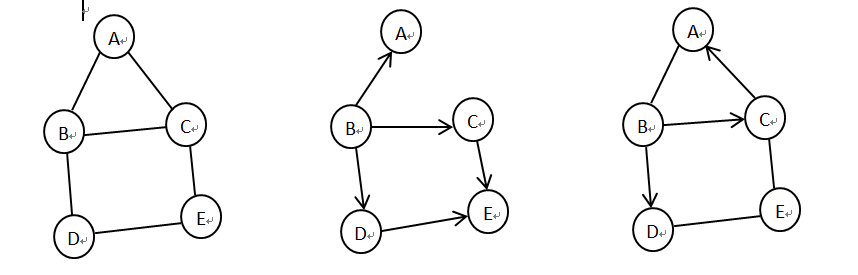
\includegraphics[scale=0.50]{1.png}
\caption{\label{graph:pdf1} An undirected graph($\emph{left}$), a directed graph ($\emph{center}$) and a partially directed graph ($\emph{right}$)}
\end{figure}

In the following we gave the definition of Bayesian network.\\
\begin{definition}
Bayesian networks are a class of graphical models that allow a concise representation of the probabilistic dependencies between a given set of random variables $\mathbf{X}$=$\{X_1,X_2,...,X_p\}$ as a directed acyclic graph (DAG) $\emph(G)=(\mathbf{V},\mathbf{A})$.Each node $\mathit{v}_i\in \mathbf{V}$
\end{definition}

The most commonly used structure learning method for Bayesian network was $\emph{Greedy search}$ algorithms. These algorithms explore the search space starting from a network strucutre (usually the empty graph) and adding, deleting, or reversing one arc at a time until the score can no longer be improved.\\
Hill-Climbing algorithm was one of the famous greedy search algorithms. we use this algorithm to do research and list the algorithm as follows:\\\\
$\mathbf{Algorithm 2.1}$ Hill- Climbing Algorithm.\\\\
1. Choose a network structure $\mathbf{G}$ over $\mathbf{V}$, usually (but not necessarily) empty.\\
2. Compute the score of $\mathbf{G}$, denoted as $Score_G$=Score(G).\\
3. Set $\emph{maxscore}$=$score_G$\\
4. repeat the following steps as long as $maxscore$ increases:\\
a. for every possible arc addition, deletion or reversal not resulting in a cyclic network:\\
i. compute the score of the modified network $G^*$ and $Score_G$=$Score_{G^*}$\\
ii.if $Score_{G^*}$ $>$ $Score_G$, set $G=G^*$ and $Score_G$=$Score_{G^*}$\\
b. update $maxscore$ with the new value of $Score_{G}$\\
5. return the directed acyclic graph $G$.\\


\section{Graphical Lasso model}

Before introduced the Graphical Lasso model, we first reviewed some knowledge of the Lasso model.

\begin{definition}
Suppose that we have data $(x^i,y_i),i=1,2,...,N$, where $x^i=(x_{i1},x_{i2},...,x_{ip})$ are the predictor variables and $y_i$ are the responses. As in the usual regression set-up, we assume either that the observations are independent or that the
$y_is$ are conditionally independent given the $x_{ij}s$. We assume that the $x_{ij}$ are standardized so that $\sum_ix_{ij}/N=0, \sum_ix_{ij}^2=1$.\\
Letting $\hat{\beta}=(\hat{\beta_1},...,\hat{\beta_p})^T$, the lasso estimate $(\hat{\alpha},\hat{\beta})$ is defined by \\

\begin{equation}
\label{}
(\hat{\alpha},\hat{\beta})=argmin{\sum_{i=1}^N(y_i-\alpha-\sum_j\beta_jx_{ij})^2}\ subject\ to \sum_j|\beta_j| \leq t\\
\end{equation}

Here $t\geq 0$ is a tuning parameter.
\end{definition}

\begin{figure}[!htb]
\centering
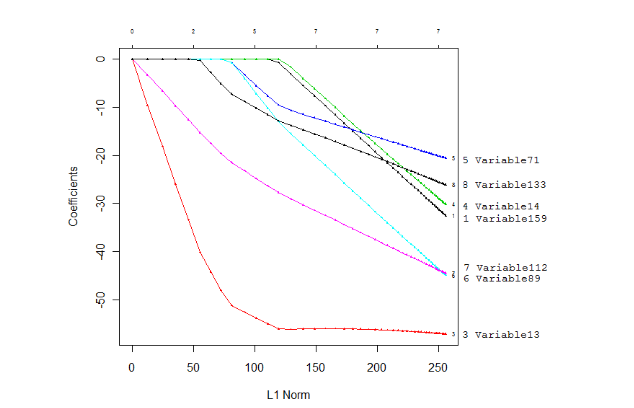
\includegraphics[scale=0.50]{2.png}
\caption{\label{graph:pdf1} The path of the Lasso model}
\end{figure}

Figure 2 showed the Lasso shrinkage of coefficients. \\

The Graphical Lasso model was introduced by Jerome Friedman, Trevor Hastie and Robert Tibshirani(2007). It proposed the estimation of sparse undirected graphical models through the use of $L_1$(lasso) regularization.\\
Suppose we have N multivariate normal observations of dimension $p$, with mean $\mu$ and covariance $\Sigma$. Let $\Theta=\Sigma^{-1}$, and let $S$ be the empirical covariance matrix, the problem is to maximize the log-likelihood:\\
\begin{equation}
log det\Theta-tr(S\Theta)-\rho|||\Theta||_1
\end{equation}

Here tr denotes the trance and $||\Theta||_1$ is the $L_1$ norm- the sum of the absolute values of the elements of $\Sigma^{-1}$. Jerome Friedman, Trevor Hastie and Robert Tibshirani used the blockwise coordinate descent approach as a launching point and proposed the Graphical lasso algoithm for the exact problem. \\
Tuo zhao and Han liu(2012) et al exploited an R package named high dimensional undirected graphs. This package used language C instead of fortran and provide functions for fitting high dimensional semiparametric Gaussian copula models.\\
Gaussian copula models extends the Gaussian graphical models by marginally transforming the variables using smooth monotone functions. \\To reduce the variance of $\hat{f}_j$, they introduced the following truncated estimator.\\
suppose we have $n$ observations for j-th variable, $x_{1j},...,x_{nj}$ and we sort all $n$ observations and get the corresponding rank $u_{1j},...,u_{nj}$. Let $\Phi$ denote the Gaussian CDF function, then we can estimate the transformed data using: \\
\begin{equation}
\hat{f}_j=\Phi^{-1}(\hat{u}_{ij})\ \
or\ \
\hat{f}_j(x_{ij})=
\begin{cases}
\Phi^{-1}(\delta)\ \ \ \ \ \ \ \ \  if \ \hat{u}_{ij}\leq\delta\\
\Phi^{-1}(\hat{u}_{ij})\ \ \ \ \ \ \  if \ \delta < \hat{u}_{ij}\leq{1-\delta}\\
\Phi^{-1}(1-\delta)\ \ \ \   if \ \hat{u}_{ij} > {1-\delta}
\end{cases}
\end{equation}

where \\

\begin{equation}
\hat{u}_{ij}=\frac{u_{ij}}{n+1}
\ \ and \ \
\delta =\frac{1}{4n^{1/4}\sqrt{\pi logn}}
\end{equation}

\section{Stock return series analysis}

During the year 2009, the world economy experienced a big depression according to the financial crisis. It raised people's awareness of the importance of risk management. To build an effective and efficient risk management system becomes more and more important. Among those risk management problems, how to build an accurate quantitative model to forecast stock return series is always a hot topic. In the past, time series prediction algorithms, such as auto Auto regressive, moving average and Garch model, performed good for stock price prediction. However there are some drawbacks in the time series model. For every time series algorithms, the stock price is assumed to be the linear combination of the past data and the error term, which was assumed to be Gaussian distribution. Through recent research, we now know the following things: 1) actual stock return distributions appear fat-tailed (compared to Normal). 2) volatility appears time- varying and clustered.3) returns are serially uncorrelated, but square returns are serially correlated.
\begin{figure}[!htb]
\centering
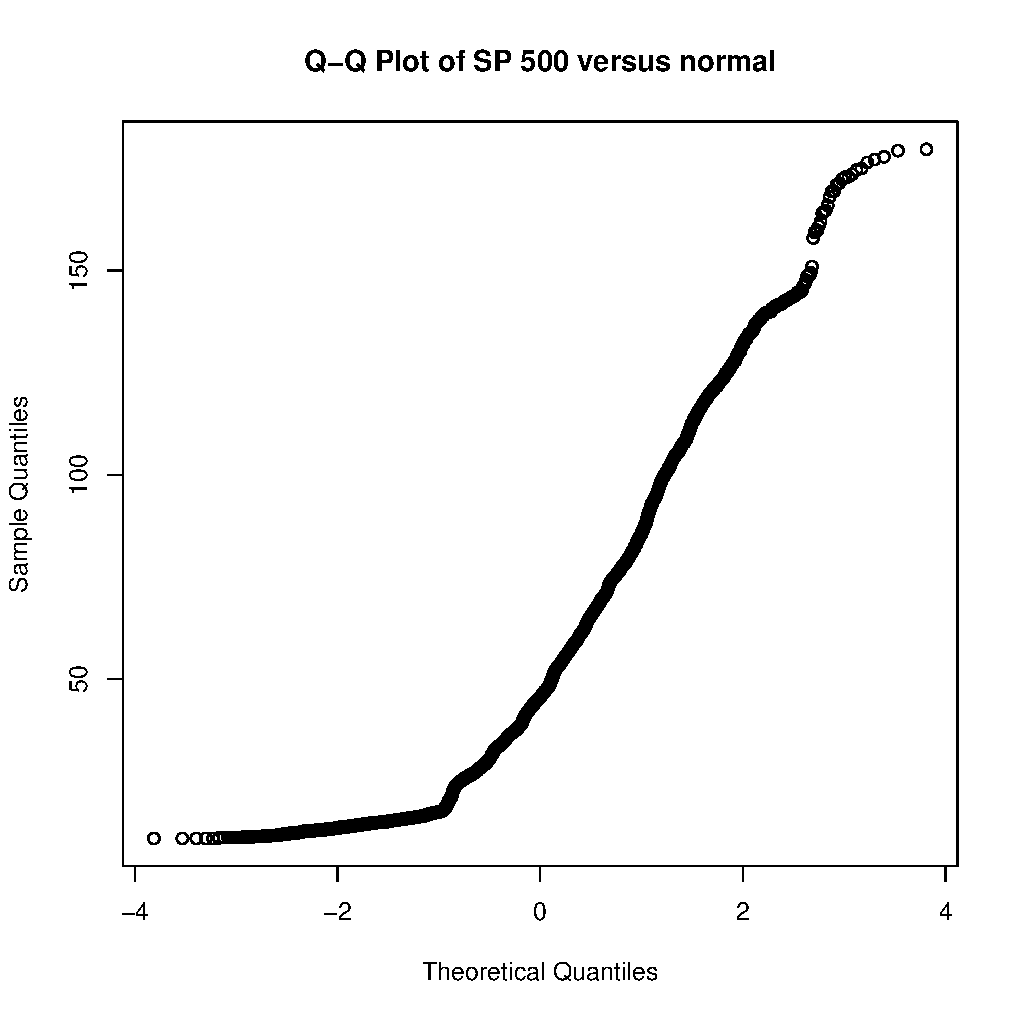
\includegraphics[scale=0.50]{sp.pdf}
\caption{\label{graph:pdf1} QQ-plot of S\&P 500 Versus normal}
\end{figure}

\begin{figure}[!htb]
\centering
\includegraphics[scale=0.50]{nasdaq.pdf}
\caption{\label{graph:pdf1} QQ-plot of Dow Versus Normal}
\end{figure}

From the above two charts, we can see that both the S\&P 500 and Dow jones indices have heavy tails than normal. \\
 According to the fat-tailed phenomenon,the time series models were not a good fit for analyze the stock returns because of their normal assumption in error terms. Bayesian network at this time became an effective weapon to overcome this difficulty. Actually, Bayesian network has already been widely used in the financial area in the recent years. For example, In Catherine Shenoy and Prakash P. Shenoy(2000), they showed how to use Bayesian networks to model portfolio risk and returns. Our research was focus on  the structure learning problem and how to use the Bayesian network to forecast the stock return series.\\
 For the Bayesian network learning process, we commonly use some greedy search methods such as Hill climbing algorithm mentioned above. However, this method typically use the random or empty graph as a start. Here we try to build the network by using hill climbing method with the help of the relationship result of Graphical Lasso model. \\

 The data we used was 452 daily closing prices from stocks in the S\&P 500. For each stock, there are 1258 observations form January 1 2003 to January 1, 2008.  We used stock return series for each stock to do analysis. The return series $r_t$ was defined as: \\
 \begin{equation}
r_t=(lnP_t-lnP_{t-1})*100
\end{equation}
where the variable $P_t$ denotes the closing price on the day $t$. \\

In Han Liu(2012), they gave us the network structure of these 452 stocks by using the package "HUGE"\\
\begin{figure}[!htb]]
\centering
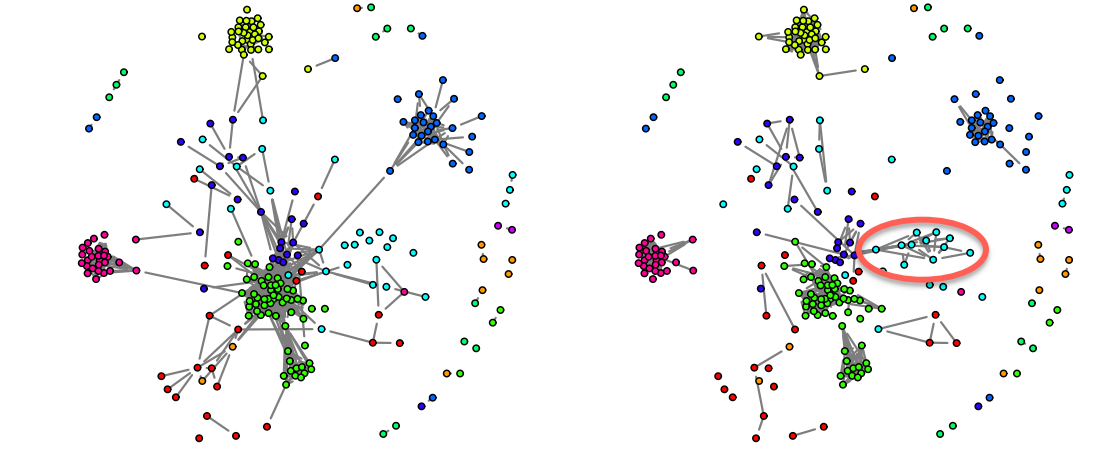
\includegraphics[scale=0.50]{huge.png}
\caption{\label{graph:pdf1} The estimated glasso (left) and nonparanormal graph(right) }
\end{figure}



Different colors in the above charts represented the different industry. The result showed that the huge package had a strong power for the high dimension problem of stock returns and the nonparanormal method performed better to reveal the relationship beyond the normality assumption.\\
our research was tried to use relationship obtained from "HUGE" package as the initial network and use Bayesian network structure learning algorithm to analyze the causal relationship among stock return series .\\
We use BIC score to compare the result of the network for the Hill climbing algorithm, Hill climbing algorithm with the help of HUGE( we call it hc.huge method) and Hill climbing algorithm with the help of HUGE.NPN(We call it hc.huge.npn method).\\
The definition of BIC score is as follows: \\

 \begin{equation}
BIC=-2ln(\hat{L})+ k*ln(n)
\end{equation}
where $\hat{L}$ is the maximum likelihood, $k$ is the number of the parameters to be estimated and $n$ is the number of data points in the observed data $x$


\begin{table}[h!]\tiny

  \caption{BIC scores for three structure learning methods}
\begin{center}
    \begin{tabular}{| c | c | c | c | c |c |c |c |c |c |c |}
    \hline
    node& 10 & 20 & 30& 40& 50& 60& 70& 80& 90& 100\\
    \hline
BIC score of hc &33853.67&64591.95&101152.7&137100.9&162166.3&197325.4&234362.4&262323.1&310709.9&336905.4\\
BIC score of hc.huge&33853.67&64591.95&101152.7&137099.1&162166.5&197322.5&234361.8&262306.3&310710.4&336897.4\\
BIC score of hc.huge.npn&33853.67&64592.4&101149.9&137106.6&162147.1&197317&234368&262294.4&310669.1&336891.4\\
\hline
\end{tabular}
  \end{center}
\end{table}

Since for each model the $k$ and $n$ were defined, so the smaller the BIC score is, the large the maximum likelihood is. We can see that from the above chart, the hc.huge.npn method performed better than hc.huge method, and hc.huge method was better than hc method itself.\\
\section{Parallel computing for Bayesian Network}
Most problems in Bayesian networks research area have a computational complexity. It means that the scales increase exponentially with the number of variables.  Hence, structure learning becomes a more and more important issue in the Bayesian network clarification area. Parallel computing is introduced here to handle this problem via using the hardware better.
In this chapter, we will provide a brief overview of the fundamental concepts and using of parallel computing. Besides, we will also show the results for using parallel computing method to deal with our stock return series analysis to see if the parallel computing method really increase the computing efficiency.

The R interpreter can only execute one command at a time, The only functions that can take advantage of multiple processors are the linear algebra routines provided by the Basic Linear ALgebra Subprograms(BLAS)library. R must be compiled against a third -party , Multi-threaded implementation of the BLAS library, such as the one provided by intel. However, performance improvements are limited to algorithms making heavy use of these routines.\\
For the Bnlearn package in R, it is designed to work with:\\
1) The snow package which provides support for simple parallel computing using the master -slave model.\\
2) The Rmpi package, which is an R interface to the c libraries implementing the \textit{Message -Passing Interface}(MPI) standard.\\
3) The rpvm package , which is designed to allow a network of heterogeneous Unix and Windows machines to be used as a single distributed parallel processor.\\
4) The \textbf{rsprng} package , which provides independent random number generators to the slaves spawned by \textbf{snow}\\

we can also apply the parallel computing method into the two phase of the Bayesian learning process:\\
The first is to structure learning process, here we use the Constraint  Based structure learning algorithms as example.\\
Constraint Based structure typically has three steps:

1)The first step  can not use the parallel method, because each d-separating set can be learned independently from the others.\\
2)The same situation holds for the second step. \\
3)The third step is sequential, because each iteration requires the status of the previous one.\\
Therefore , the information available to the slave processes has to be synchronized only collected is between the first and the second step and between the second and the third step.\\
We will now examine the practical implications of parallelizing a constraint -based learning algorithm. The dataset we use is the \textit{hailfinder} included in the \textbf{bnlearn} package. It contains 56 variables and 20000 observations and is large enough to properly highlight the advantages and the limitations of parallel computing.\\
The R language example which use the two slaves process is as follows:\\
>data(hailfinder)
>c1=makeCluster(2,type="MPI")
>res= gs(hailfinder,cluster = c1)
>unlist (clusterEvalQ(c1,.test.counter))
>.test.counter
>stopCluster(c1)   


\section{Conclusion}
Bayesian network now is widely used in the financial area, such as risk management and stock return forecasting. It can gave us the stochastic dependency among random variables via an acyclic directed graph. It can overcome the drawback of time series model because this model did not depend on the assumption of normal distribution. In our research, we try to find the causal relationship among the stock return series by Bayesian network. we applied the results of "HUGE" model into our structure learning algorithm. Through comparing the BIC scores, it showed that the hc.huge.npn method is best followed by hc.huge method and the hc method itself is the worst.



\end{document}
